%%%% CS553 Cryptography Term Paper TEMPLATE %%%%\and

%%%% 1. DOCUMENTCLASS %%%%
\documentclass[preprint]{transcrypto}
%%%% NOTES:
% - Change "submission" to "final" for final version
% - Add "spthm" for LNCS-like theorems


%%%% 2. PACKAGES %%%%
\usepackage{lipsum} % Example package -- can be removed
\usepackage{algorithm}%
\usepackage{hyperref}
\hypersetup{
    colorlinks=black,
    linkcolor=black,
    filecolor=black,      
    urlcolor=black,
}
\usepackage{xcolor}
% http://ctan.org/pkg/algorithms
\usepackage{algpseudocode}% http://ctan.org/pkg/algorithmicx
\newcommand{\TeaserImage}[1]{\vcenter{\hbox{\includegraphics[height=1in]{#1}}}}
%%%% 3. AUTHOR, INSTITUTE %%%%
\author{Anmol Sagar\inst{1}\and Ashutosh Garg\inst{2}\and Prince Kumar Pansari\inst{3}}
\institute{
  IIT Bhilai, Raipur, India, \email{anmols@iitbhilai.ac.in}
  \and
  IIT Bhilai, Raipur, India, \email{ashutoshg@iitbhilai.ac.in}
  \and
  IIT Bhilai, Raipur, India, \email{princep@iitbhilai.ac.in}
}
%%%% NOTES:
% - We need a city name for indexation purpose, even if it is redundant
%   (eg: University of Atlantis, Atlantis, Atlantis)
% - \inst{} can be omitted if there is a single institute,
%   or exactly one institute per author


%%%% 4. TITLE %%%%
\title{Loong: A Family of Involutional Lightweight Block Cipher}
%%%% NOTES:
% - If the title is too long, or includes special macro, please
%   provide a "running title" as optional argument: \title[Short]{Long}
% - You can provide an optional subtitle with \subtitle.

\begin{document}

\maketitle


%%%% 5. KEYWORDS %%%%
\keywords{Block Cipher \and Lightweight Cryptography \and Involution \and Substitution Permutation Network \and Similar Encryption Decryption Process \and Save Resources}


%%%% 6. ABSTRACT %%%%
\begin{abstract}
  
In the past few years, Cryptography scientists are mainly focusing on lightweight ciphers because the field of Internet of Things (IoT) has grown fast from the last few years and uses of them will grow as time passes. The IoTs cannot use ciphers like AES that although very secure because it needs more power and resources that is an issue with them. So, the main concern behind lightweight is to use less power and resources, and provide as much security as ciphers like AES provide.\\
Block ciphers mainly have two structures, SPN based and Feistel Network based. The SPN structure has been widely used in the design of block cipher. However, the algorithm of encryption and decryption in the SPN network is different. Loong is a block cipher that is based on SPN structure. The design of Loong is such that it can use the same implementation for both encryption and decryption. Thus it is very easy to implement on software as well as hardware. The direction of input and output is the same for both encryption and decryption.
Rigorous analysis indicates that Loong is of high security against cryptanalysis, especially the differential attack and linear attack. Those facts are based on proper experiments and comparisons. As Loong is easy to implement that makes it more suitable for hardware implementation or IoT, so it is a tough competitor with other lightweight ciphers like PRESENT, TEA etc. 
\end{abstract}


%%%% 7. PAPER CONTENT %%%%
\section{Introduction}
Block Cipher is the effective method for resisting adversarial attempts to read data, it is an efficient method to store the data as well as transit on the network. It is one the two common modern symmetric cipher types. It is different from the stream cipher because it deals with the data in chunks. One of the most efficient block ciphers that we are using right now is Advanced Encryption Standard(AES). It is the one of the most famous cipher approved by U.S. Government to protect electronic data, and certified in 2001.\\
Although AES is one of the most secure ciphers and no-one breaks it till now, research is still going on in the field of cryptography because in this new era we need security in small devices that are called IoT devices. These devices are very useful but in terms of resources and power they have their own limitations. It is said that Security comes at the cost of computation and it's easy to understand. In today's time IoT devices are everywhere, Institutes and militaries are using RFID tags and smart cards. Mobile devices like smart watches, tablets have become a part of daily life. Armies are using drones as their secret weapon. So all these devices are fully content with highly confidential information that can affect some one or many ones life. But if we use a heavy-weight cipher then that consumes power very early. So in today's time most of the research are going on in the lightweight ciphers.\\
In last few years many of the block ciphers had developed and still development is going on some of the famous Lightweight block ciphers PRESENT, TEA and so on.\\
Block cipher mainly has two structures, SPN based and Feistel Network. One of the famous examples of Feistel networks is DES(Data Encryption Standard), The advantage of Feistel Network is the process to encrypt and decrypt the data is the same. But Feistel Network makes diffusion of the half block in each round so to make the block secure we need too many rounds that make it inefficient. That's why people majorly uses SPN because it provides 
more efficiency then Feistel but hard to implement on hardware because it uses different encryption and decryption processes.\\
AES is one of the best SPN block ciphers but it has some limitations, (1) It's costly to make two different circuits on hardware for encryption and decryption. (2) It is not useful for smart cards because they have very less memory to store data. Therefore, It is much needed to make a cipher like SPN that have similar encryption and decryption processes.\\
\section{Specification of Loong}
Loong Cipher is SPN based cipher. There are three members of Loong Cipher each with a block size of 64 bits, but three different key lengths: 64, 80 and 128 bits. The round numbers are 16 for 64 bit key, 20 for 80 bits and 32 for 128 bits. The members of Loong are denoted as \textbf{Loong-64}, \textbf{Loong-80} and \textbf{Loong-128} on the basis of length of the keys.


\section{Encryption}
In encryption, the 64-bit block of plaintext and the primary key is regarded as input. The size of primary key can be 64-bit, 80-bit or 128-bit. 
The round function of Loong includes AddRoundKey operation, SubCell operation, MixRow operation and MixColumn operation. The encryption process of Loong Cipher is given in Figure \ref{figure:encryption}.\\
The encryption function of Loong can be expressed as:
\begin{equation}
    ENC_{RN} = ARK(RK, RC^{0}) \circ (\bigcirc_{r = 1}^{RN} SC \circ MR \circ MC \circ SC \circ ARK(RK, RC^{RN}))
\end{equation}
\begin{figure}[H]
	\centering
	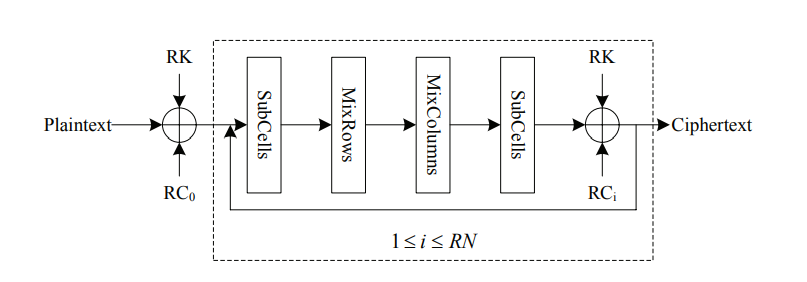
\includegraphics[width=12cm]{encrypt.png}
	\caption{Encryption in Loong}
	\label{figure:encryption}
\end{figure}
The algorithm \ref{alg:encryption} illustrates the $ENC_{RN}$ equation given earlier, where the input to the algorithm is plaintext and round key and the output is ciphertext.
\begin{algorithm}[H]
    \caption{Encryption Algorithm}
    \label{alg:algorithm-label}
    \begin{algorithmic}
        \item $ENC_{RN}$
        \item \textbf{Input :} Plaintext, RK(Round Key);
        \item \textbf{Output: } Ciphertext;
        \item 01: state $\leftarrow$ Plaintext;
        \item 02: AddRoundKey(state, RK, RC);
        \item 03: for i = 1 to RN do
        \item 04: \qquad SubCell(state);
        \item 05: \qquad MixRow(state);
        \item 06: \qquad MixColumn(state);
        \item 07: \qquad SubCell(state);
        \item 08: \qquad AddRoundKey(state, RK, RC);
        \item 09: endfor
        \item 10: Ciphertext $\leftarrow$ state;
        \item 11: \textbf{Return} Ciphertext;
    \end{algorithmic}
    \label{alg:encryption}
\end{algorithm}


\subsection{Subcell}
The Subcell operation is used to provide confusion. It means this operation is used to obscure the relationship between the plaintext and the ciphertext. In this operation, we use a S-Box which performs substitution. Since, in loong we work on 4bit nibbles, so possible values for nibbles are 0 to E. So, the S-Box contains 16 elements. The S-Box is given in the Table \ref{table:sbox}.
\begin{table}[H]
	\begin{center}
	\begin{tabular}{||c||c|c|c|c|c|c|c|c|c|c|c|c|c|c|c|c|}
		\hline
		x & 0 & 1 & 2 & 3 & 4 & 5 & 6 & 7 & 8 & 9 & A & B & C & D & E & F\\ 
		\hline
		S(x) & C & A & D & 3 & E & B & F & 7 & 9 & 8 & 1 & 5 & 0 & 2 & 4 &6\\
		\hline
	\end{tabular}
	\end{center}
	\caption{S-Box}
	\label{table:sbox}
\end{table}
There is a special property of \textbf{involutive} in the SBox of loong cipher. It means that the SBox is its own inverse. The same property is illustrated in the Table \ref{table:involutive}.
\begin{table}[H]
	\begin{center}
	\begin{tabular}{||c||c||c||}
		\hline
		x & S(x) & S(S(x)) \\ 
		\hline
		0 & C & 0 \\
		\hline
		1 & A & 1\\
		\hline
		2 & D & 2\\
		\hline
		3 & 3 & 3\\
		\hline
		4 & E & 4\\
		\hline
		5 & B & 5\\
		\hline
		6 & F & 6\\
		\hline
		7 & 7 & 7\\
		\hline
		8 & 9 & 8\\
		\hline
		9 & 8 & 9\\
		\hline
		A & 1 & A\\
		\hline
		B & 5 & B\\
		\hline
		C & 0 & C\\
		\hline
		D & 2 & D\\
		\hline
		E & 4 & E\\
		\hline
		F & 6 & F\\
		\hline
	\end{tabular}
	\end{center}
	\caption{x = S(S(x))}
	\label{table:involutive}
\end{table}


\subsection{MixRow}
The MixRow Operation is used to provide better diffusion. In MixRow Operation, the state is post-multiplied by a diffusion matrix $M$. The matrix multiplication is performed in finite field $GF(2^4)$ where the irreducible polynomial is $x^4 + x+ 1$.\\\\
The matrix multiplication operation of the MixRow is as follows:\\
\begin{equation}
state \leftarrow 
\begin{pmatrix}
state_0 & state_1 & state_2 & state_3 \\
state_4 & state_5 & state_6 & state_7 \\
state_8 & state_{9} & state_{10} & state_{11} \\
state_{12} & state_{13} & state_{14} & state_{15}
\end{pmatrix}
\times
\begin{pmatrix}
1 & 4 & 9 & 13\\
4 & 1 & 13 & 9\\
9 & 13 & 1 & 4\\
13 & 9 & 4 & 1
\end{pmatrix}
\end{equation}



\subsection{MixColumn}
The MixColumn Operation is also used to provide better diffusion. In MixColumn Operation, the state is pre-multiplied by a diffusion matrix $M^'$. The matrix multiplication is performed in finite field $GF(2^4)$ where the irreducible polynomial is $x^4 + x+ 1$.\\\\
The matrix multiplication operation of the MixColumn is as follows:\\
\begin{equation}
state \leftarrow 
\begin{pmatrix}
13 & 9 & 4 & 1\\
9 & 13 & 1 & 4\\
4 & 1 & 13 & 9\\
1 & 4 & 9 & 13
\end{pmatrix}
\times
\begin{pmatrix}
state_0 & state_1 & state_2 & state_3 \\
state_4 & state_5 & state_6 & state_7 \\
state_8 & state_{9} & state_{10} & state_{11} \\
state_{12} & state_{13} & state_{14} & state_{15}
\end{pmatrix}
\end{equation}



\subsection{Round Constants}
The round constants of this cipher is of 6-bit. It can be denoted as $(rc_5, rc_4, rc_3, rc_2, rc_1, rc_0)$ It is generated by the 6-bit affine linear-feedback shift register(LFSR).\\
The update function is defined as:
\begin{equation}
    (rc_5, rc_4, rc_3, rc_2, rc_1, rc_0) \leftarrow (rc_4, rc_3, rc_2, rc_1, rc_0, rc_5 \oplus rc_4 \oplus 1)
\end{equation}
The round constants are initialized to zero, means all the 6-bits are 0. And it is updated before using in a given round with the update function defined earlier.\\
The Table \ref{table:roundconstant} is the pre-computed element of round constants of all the rounds.
\begin{table}[h!]
	\begin{center}
	\begin{tabular}{c| c c c c c c c c c c c}
	    \hline
	    Rounds & \multicolumn{11}{c}{Constants}\\
		\hline
		0-10 & 01 & 03 & 07 & 0F & 1F & 3E & 3D & 3B & 37 & 2F & 1E\\
		11-21 & 3C & 39 & 33 & 27 & 0E & 1D & 3A & 35 & 2B & 16 & 2C\\
		22-32 & 18 & 30 & 21 & 02 & 05 & 0B & 17 & 2E & 1C & 38 & 31\\
		\hline
	\end{tabular}
	\end{center}
	\caption{Elements of Round Constants}
	\label{table:roundconstant}
\end{table}\\
Loong has three diiferent key blocks with 16, 20 and 32 rounds respectively. Round Constant are used in AddRoundKey operation of every round and there is also one extra AddRoundKey operation earlier. So, 17, 21 and 33 different round constants are required for three different key size respectively.\\ 
The adding(XOR) of the round constants in the AddRoundKey is arranged as follows: 
\begin{center}
    $\begin{bmatrix}
0 & 0 & 0 &(rc_5 || rc_4 || rc_3)\\
0 & 0 & 1 &(rc_2 || rc_1 || rc_0)\\
0 & 0 & 2 &(rc_5 || rc_4 || rc_3)\\
0 & 0 & 4 &(rc_2 || rc_1 || rc_0)
\end{bmatrix}$
\end{center}




\subsection{AddRoundKey}
Loong has three different key length which are 64-bit, 80-bit and 128-bit. The 64-bit key is written as $k_0, k_1, ..., k_{15}$, the 80-bit key is written as $k_0, k_1, ..., k_{19}$ and the 128-bit key is written as $k_0, k_1, ..., k_{31}$.\\
The 64-bit key of Loong-64 is arranged into a round key matrix as:\\
\begin{center}
$ RK \leftarrow 
\begin{bmatrix}
k_0 & k_1 & k_2 & k_3 \\
k_4 & k_5 & k_6 & k_7 \\
k_8 & k_9 & k_{10} & k_{11} \\
k_{12} & k_{13} & k_{14} & k_{15}
\end{bmatrix}$
\end{center}
The 80-bit key of Loong-80 is arranged into two round key matrix as:\\
\begin{center}
$ RK_0 \leftarrow 
\begin{bmatrix}
k_0 & k_1 & k_2 & k_3 \\
k_4 & k_5 & k_6 & k_7 \\
k_8 & k_9 & k_{10} & k_{11} \\
k_{12} & k_{13} & k_{14} & k_{15}
\end{bmatrix} \hspace{1cm}
RK_1 \leftarrow 
\begin{bmatrix}
k_{16} & k_{17} & k_{18} & k_{19}\\
k_0 & k_1 & k_2 & k_3 \\
k_4 & k_5 & k_6 & k_7 \\
k_8 & k_9 & k_{10} & k_{11}
\end{bmatrix}$
\end{center}
The 128-bit key of Loong-128 is arranged into two round key matrix as:\\
\begin{center}
$ RK_0 \leftarrow 
\begin{bmatrix}
k_0 & k_1 & k_2 & k_3 \\
k_4 & k_5 & k_6 & k_7 \\
k_8 & k_9 & k_{10} & k_{11} \\
k_{12} & k_{13} & k_{14} & k_{15}
\end{bmatrix} \hspace{1cm}
RK_1 \leftarrow 
\begin{bmatrix}
k_{16} & k_{17} & k_{18} & k_{19}\\
k_{20} & k_{21} & k_{22} & k_{23} \\
k_{24} & k_{25} & k_{26} & k_{27} \\
k_{28} & k_{29} & k_{30} & k_{31}
\end{bmatrix}$
\end{center}
For 64-bit key, the AddRoundKey operation is as:
\begin{equation}
    state \leftarrow state \oplus RK \oplus RC_{i} \hspace{10pt}
    (0 \leq i \leq RN)     
\end{equation}
For 80-bit and 128-bit key, the AddRoundKey Operation is as:\\
\begin{equation}
    state \leftarrow state \oplus RK_{i\;mod\;2} \oplus RC_{i}
    \hspace{10pt}
    (0 \leq i \leq RN) 
\end{equation}




\section{Decryption}
The decryption algorithm in loong cipher is same as the encryption. Means the direction of input and output data are same for both encryption and decryption. The only difference with the encryption is that here the round constants are used in reverse order.\\\\
The decryption function of Loong can be expressed as:
\begin{equation}
    DEC_{RN} = ARK(RK, RC^{RN}) \circ (\bigcirc_{r = RN-1}^{0} SC \circ MR \circ MC \circ SC \circ ARK(RK, RC^0))
\end{equation}
Since, the algorithm of encryption and decryption is same, decryption can reuse the implementation of the encryption in both hardware and software. It uses less resource(memory) to implement, so it will be very easy to implement in hardware.
\begin{figure}[H]
	\centering
	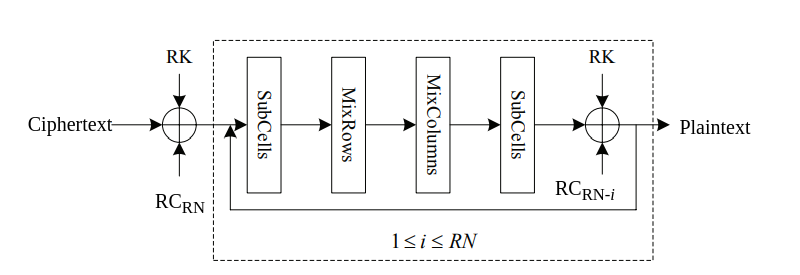
\includegraphics[width=12cm]{decrypt.png}
	\caption{Decryption in Loong}
\end{figure}



\section{Observations}
\subsection{DDT-Difference Distribution Table}
As we can see from the DDT Table \ref{table:ddt},the highest value (except 16, where input both input and output difference is 0) is 4.\\
Therefore, the maximum differential probability of the SBox is \scalebox{1.3}{$\frac{4}{16}$ = $\frac{1}{4}$}\\
\begin{table}[H]
	\begin{center}
	\begin{tabular}{||c||c|c|c|c|c|c|c|c|c|c|c|c|c|c|c|c|c|}
	    \hline
	    I/O & 0 & 1 & 2 & 3 & 4 & 5 & 6 & 7 & 8 & 9 & 10 & 11 & 12 & 13 & 14 & 15\\
		\hline
		\hline
		0 & 16 &  - &  - &  - &  - &  - &  - &  - &  - &  - &  - &  - &  - &  - &  - &  - \\
        \hline
        1 &  - & 2 & 4 &  - & 2 & 2 & 2 &  - & 2 &  - &  - &  - &  - &  - & 2 &  - \\
        \hline
        2 &  - & 4 &  - &  - & 4 &  - &  - &  - & 2 & 2 &  - &  - & 2 & 2 &  - &  - \\
        \hline
        3 &  - &  - &  - &  - & 2 &  - & 4 & 2 &  - & 4 &  - &  - & 2 &  - &  - & 2 \\
        \hline
        4 &  - & 2 & 4 & 2 & 2 & 2 &  - &  - &  - & 2 & 2 &  - &  - &  - &  - &  - \\
        \hline
        5 &  - & 2 &  - &  - & 2 &  - &  - & 4 & 2 &  - & 2 & 2 & 2 &  - &  - &  - \\
        \hline
        6 &  - & 2 &  - & 4 &  - &  - &  - & 2 & 2 &  - &  - &  - &  - & 4 & 2 &  - \\
        \hline
        7 &  - &  - &  - & 2 &  - & 4 & 2 &  - &  - &  - &  - & 2 & 2 & 2 &  - & 2 \\
        \hline
        8 &  - & 2 & 2 &  - &  - & 2 & 2 &  - &  - & 2 &  - & 2 & 2 &  - & 2 &  - \\
        \hline
        9 &  - &  - & 2 & 4 & 2 &  - &  - &  - & 2 & 2 &  - & 2 & 2 &  - &  - &  - \\
        \hline
        10 &  - &  - &  - &  - & 2 & 2 &  - &  - &  - &  - & 2 & 2 &  - & 4 &  - & 4 \\
        \hline
        11 &  - &  - &  - &  - &  - & 2 &  - & 2 & 2 & 2 & 2 & 2 &  - & 2 &  - & 2 \\
        \hline
        12 &  - &  - & 2 & 2 &  - & 2 &  - & 2 & 2 & 2 &  - &  - & 2 &  - & 2 &  - \\
        \hline
        13 &  - &  - & 2 &  - &  - &  - & 4 & 2 &  - &  - & 4 & 2 &  - &  - & 2 &  - \\
        \hline
        14 &  - & 2 &  - &  - &  - &  - & 2 &  - & 2 &  - &  - &  - & 2 & 2 & 2 & 4 \\
        \hline
        15 &  - &  - &  - & 2 &  - &  - &  - & 2 &  - &  - & 4 & 2 &  - &  - & 4 & 2 \\
        \hline
	\end{tabular}
	\end{center}
	\caption{DDT of S-Box}
	\label{table:ddt}
\end{table}

\subsection{LAT-Linear Approximation Table}
The highest absolute value observed in the LAT Table \ref{table:lat} is 4(ignoring the point where alpha and beta is zero) indicating it occurs with probability \scalebox{1.3}{$\frac{12}{16}$ = $\frac{3}{4}$}. 
\begin{table}[H]
	\begin{center}
	\begin{tabular}{||c||c|c|c|c|c|c|c|c|c|c|c|c|c|c|c|c|c|}
	    \hline
	    I/O & 0 & 1 & 2 & 3 & 4 & 5 & 6 & 7 & 8 & 9 & 10 & 11 & 12 & 13 & 14 & 15\\
		\hline
		\hline
        0 & 8 & - & - & - & - & - & - & - & - & - & - & - & - & - & - & - \\
        \hline
        1 & - & - & 4 & - & -2 & -2 & 2 & -2 & -2 & 2 & 2 & 2 & 4 & - & - & - \\
        \hline
        2 & - & 4 & - & - & 4 & - & - & - & -4 & - & - & - & - & 4 & - & - \\
        \hline
        3 & - & - & - & - & -2 & -2 & 2 & 2 & 2 & -2 & -2 & 2 & - & 4 & - & 4 \\
        \hline
        4 & - & -2 & 4 & -2 & 2 & - & -2 & - & -2 & -4 & -2 & - & - & -2 & - & 2 \\
        \hline
        5 & - & -2 & - & -2 & - & -2 & - & -2 & - & 2 & -4 & -2 & - & 2 & 4 & -2 \\
        \hline
        6 & - & 2 & - & 2 & -2 & - & 2 & -4 & -2 & - & -2 & - & -4 & -2 & - & 2 \\
        \hline
        7 & - & -2 & - & 2 & - & -2 & -4 & -2 & - & 2 & - & -2 & - & 2 & -4 & 2 \\
        \hline
        8 & - & -2 & -4 & 2 & -2 & - & -2 & - & -4 & -2 & - & 2 & 2 & - & 2 & - \\
        \hline
        9 & - & 2 & - & -2 & -4 & 2 & - & 2 & -2 & - & -2 & -4 & 2 & - & -2 & - \\
        \hline
        10 & - & 2 & - & -2 & -2 & -4 & -2 & - & - & -2 & 4 & -2 & -2 & - & 2 & - \\
        \hline
        11 & - & 2 & - & 2 & - & -2 & - & -2 & 2 & -4 & -2 & - & 2 & - & -2 & -4 \\
        \hline
        12 & - & 4 & - & - & - & - & -4 & - & 2 & 2 & -2 & 2 & 2 & -2 & 2 & 2 \\
        \hline
        13 & - & - & 4 & 4 & -2 & 2 & -2 & 2 & - & - & - & - & -2 & 2 & 2 & -2 \\
        \hline
        14 & - & - & - & - & - & 4 & - & -4 & 2 & -2 & 2 & -2 & 2 & 2 & 2 & 2 \\
        \hline
        15 & - & - & - & 4 & 2 & -2 & 2 & 2 & - & - & - & -4 & 2 & -2 & 2 & 2 \\
        \hline
	\end{tabular}
	\end{center}
	\caption{LAT of S-Box}
	\label{table:lat}
\end{table}

\subsection{Diffusion Spread in Loong}
Here you can observe that if one bit is differ in two different states, then how the difference or diffusion spread in the whole 64-bit block,
\begin{center}
      $\TeaserImage{a1b.png} \xrightarrow{\text{SC}} \TeaserImage{a1b.png}
        \xrightarrow{\text{MixRow}} \TeaserImage{3.png} $
        $\xrightarrow{\text{MixColumn}}
        \TeaserImage{a1d.png} \xrightarrow{\text{SC}}\TeaserImage{a1d.png}$
 \end{center}
So after one round diffusion spread in whole 64-bit block.






\section{SECURITY ANALYSIS}
\subsection{DIFFERENTIAL ATTACK AND LINEAR ATTACK}
For differential attack maximum differential characteristic probability is small enough,
the cipher can resist differential cryptanalysis and the differential characteristic probability
upper bound often can be calculated by the number of active S-boxes, So if we find total number of active S-Box then we can comment Differential attack.\\\\
To calculate the minimum number of active S-Box we construct mixed integer linear programming that is also called as MILP. Round Function process can be represented  as : SubCells $\rightarrow$ MixRows $\rightarrow$ MixColumns $\rightarrow$ SubCells. Changes of the first round  of loong can be represented as follows. Every variable x  as a nibble of Loong state. If the difference is non-zero, the variable x is 1, otherwise, x is 0. all variable are represent input of the subcell so equation are summed in the objective function which basically represent active S-Box. \\\\
The MixRows and MixColumns are linear functions and have
differentials. The linear branch number of the MixRows and
MixColumns is 5. We use linear equations to describe the
input and output difference and linear mask vectors MixRows
and MixColumns operations. \\\\
\begin{center}
    \scalebox{1}{$\begin{bmatrix} x_0 & x_4 & x_8 & x_{12}\\ x_1 & x_5 & x_9 & x_{13}\\
     x_2 & x_6 & x_{10} & x_{14}\\ x_3 & x_7 & x_{11} & x_{15} \end{bmatrix}$
    $\xrightarrow{\text{SC}}$
    $\begin{bmatrix} x_0 & x_4 & x_8 & x_{12}\\ x_1 & x_5 & x_9 & x_{13}\\
    x_2 & x_6 & x_{10} & x_{14}\\ x_3 & x_7 & x_{11} & x_{15} \end{bmatrix}$
    $\xrightarrow{\text{Mix Row}}$
    $\begin{bmatrix} x_{16} & x_{17} & x_{18} & x_{19}\\ x_{20} & x_{21} & x_{22} & x_{23}\\
    x_{24} & x_{25} & x_{26} & x_{27}\\ x_{28} & x_{29} & x_{30} & x_{31} \end{bmatrix}$} \\
    
    \vspace{20pt}
    \scalebox{1}{
    $\xrightarrow{\text{Mix Column}}$
    $\begin{bmatrix} x_{32} & x_{36} & x_{40} & x_{44}\\ x_{33} & x_{37} & x_{41} & x_{45}\\
    x_{34} & x_{38} & x_{42} & x_{46}\\ x_{35} & x_{39} & x_{43} & x_{47} \end{bmatrix}$
    $\xrightarrow{\text{SC}}$
    $\begin{bmatrix} x_{32} & x_{36} & x_{40} & x_{44}\\ x_{33} & x_{37} & x_{41} & x_{45}\\
    x_{34} & x_{38} & x_{42} & x_{46}\\ x_{35} & x_{39} & x_{43} & x_{47} \end{bmatrix}$}
    
\end{center}
\vspace{10pt}
The MixRows can be constrained by the following linear equations:
\begin{gather}
    x_0+x_1+x_2+x_3+x_{16}+x_{20}+x_{24}+x_{28}-5d_0 \ge0\\
    x_4+x_5+x_6+x_7+x_{17}+x_{21}+x_{25}+x_{29}-5d_1\ge0\\
    x_8+x_9+x_{10}+x_{11}+x_{18}+x_{22}+x_{26}+x_{30}-5d_2\ge0\\
    x_{12}+x_{13}+x_{14}+x_{15}+x_{19}+x_{23}+x_{27}+x_{31}-5d_3\ge0
\end{gather}
The MixColumns can be constrained by the following linear equations:
\begin{gather}
    x_{16}+x_{17}+x_{18}+x_{19}+x_{32}+x_{33}+x_{34}+x_{35}-5d_4\ge0\\
    x_{20}+x_{21}+x_{22}+x_{23}+x_{36}+x_{37}+x_{38}+x_{39}-5d_5\ge0\\
    x_{24}+x_{25}+x_{26}+x_{27}+x_{40}+x_{41}+x_{42}+x_{43}-5d_6\ge0\\
    x_{28}+x_{29}+x_{30}+x_{31}+x_{44}+x_{45}+x_{46}+x_{47}-5d_7\ge0
\end{gather}
From above Equation we get minimum number of differential or linear active S-boxes for n rounds of Loong is 8n, after first round minimum 8 S-Box are active, after first round minimum 32 S-Box are active.\\
The S-box of Loong have maximal probability of a differential is $2^{−2}$ and the maximal absolute bias of a linear approximation
is $2^{−2}$ . For Loong, it's 9-round differential probability is $2^{-144}$ and its 9-round bias of linear probability is $2^{-73}$ .\\
Loong-64 has 16 rounds, and its differential probability is $2^{-256}$
and its bias of linear probability is $2^{-129}$ .\\
Loong-80 has 20 rounds, and its differential probability is $2^{-320}$ and its bias
of linear probability is $2^{-161}$ .\\
And Loong-128 has 32 rounds, and its differential probability is $2^{-512}$ and its bias of linear
probability is $2^{-257}$ .\\ Therefore, Loong has high security and
we believe Loong is enough to resist against differential and
linear attacks.

\subsection{RELATED-KEY ATTACK}
In this analyze the probability of related-key differential characteristics. For 64-bit key version. The 64-bit primary key is round key. When the differences are inserted in the round key input,the round key will be active in Loong-64.
 \begin{center}
      $\TeaserImage{a1b.png} \xrightarrow{\text{SC}} \TeaserImage{a1b.png}
        \xrightarrow{\text{MixRow}} \TeaserImage{3.png} $
        $\xrightarrow{\text{MixColumn}}
        \TeaserImage{a1d.png} \xrightarrow{\text{SC}}\TeaserImage{a1d.png}$
 \end{center}
 After  obtaining related-key differential path, they are
 ensured that at least one round is active in every two rounds
 by this method. So Loong-64 has at least (RN /2) $\times$ 8 active
 S-boxes in related-key differential path, and its 8-round differential probability is $2^{-64}$ . Overall, the differential probability of Loong-64 is $2^{-128}$ \\
 Hence it's secure under related-key attacks.\\
 
\subsection{ALGEBRAIC ATTACK}
The Algebraic attacks are based on the deducing the secret key by solving the nonlinear equations that involves key bits, cipher-text and  plain-text. This is based on the major work of \textbf{Shannon}.\\
In the Algebraic attack we deal with two phases:
\begin{enumerate}
    \item Analyzed sufficiently enough low-degree or multivariate nonlinear equation.
    \item Recover the key by solving the equation.
\end{enumerate}
For the \textit{Loong} non-linear component is Sub-Cell or you can say s-box. for each round of \textit{Loong} you are using sub-cell two times and each sub-cell uses 16 s-boxes that leads to 32 s-boxs in each round. Here, A intresting result that we have is '\textit{A 4 × 4 S-box can be described by 21 quadratic equations of 8 input/output-bit variables over}'\footnote{N. T. Courtois and J. Pieprzyk, ‘‘Cryptanalysis of block ciphers with
overdefined systems of equations,’’ in Proc. 8th Int. Conf. Theory Appl.
Cryptol. Inf. Secur., vol. 2501, 2002, pp. 267–287}.\\
For, Loong-64 has 512 sbox after 16 rounds of encryption. similarly, Loong-80 has 640 s-boxes after 20 round and Loong-128 has 1024 s-boxes after 32 round of encryption. Therefore Loong-64 can be described as 10752 quadratic equa-
tions of 4096 variables, the Loong-80 can be described as 13440 quadratic equations of 5120 variables and the Loong-128 can be describe as 21504 quadratic equations of 8192 variables. Here is the comparison of Loong with other lightweight cipher. \\
\begin{table}[h!]
\centering
\begin{tabular}{ |c|c|c|c|c|  }
\hline
\multicolumn{5}{|c|}{The algebraic comparison information in different ciphers} \\
\hline
Ciphers &Rounds &S-boxes &Quadratic equations &Variables\\
\hline
Loong-64 &16 &512 &10752    &4096\\
Loong-80 &20 &\textbf{640} &\textbf{13440} &\textbf{5120}\\
Loong-128 &32 &\textbf{1024} &\textbf{21504} &\textbf{8192}\\
KLEIN-64 &12 &240 &5040 &1920\\
MIBS-80 &32 &320 &6720 &2560\\
PRESENT-80 &31 &527 &11067 &4216\\
\hline
\end{tabular}
\caption{Algebraic Comparison in Differnet Ciphers}
\label{table:algebra}
\end{table}
From the comparison table \ref{table:algebra} you can conclude that Loong is getting much better results compare to other lightweight ciphers. You can see that if you can break Loong-80 from algebric attack then you can break PRESENT-80 That is still one of the best lightweight cipher.\\

\subsection{MEET-IN-THE-MIDDLE ATTACK}
The Meet in the middle is one of the known-plaintext attack. It is based on the trade-off between time and memory that also rely on performing multiple encryption oprations in sequence.\\
For the Loong Diffusion is faster, and after 2 round it spread in each cell, The block of 64 bit is fully defused. So the number of round used in Partial matching is 3(2*Number of round to defused - 1 = 2*2 -1 = 3). It is part of the intermediate state as it uses alot more then 3 rounds. you can not get the primary key by this process too. With the splice and cut technique, meet in the middle attack can alalyze upto 7 rounds That it worst case for now. Therefore, Loong is safe for this attack for now.  
%%%% 8. BILBIOGRAPHY %%%%


\section{Conclusion}
In this paper, we \textbf{YAnonymous} studied Loong which is a Lightweight Block cipher based on SPN structure. The S-Box of the Loong is involutional in nature, which means that the S-Box is its own inverse. The round transformation of the Loong are also involutional, which makes both the encryption and decryption process same. The decryption process of the Loong can simply use the codes and circuitries of the encryption process to save resources in both the software and hardware implementation. Since, the Round Function of Loong has two subcell operations which makes the more active S-Box compared to its competitors Lightweight block ciphers. Since, it has more active S-Box, so it will also provide better confusion which means there is a obscure relationship between the plaintext and the ciphertext.\\
From the cryptoanalysis perspective Loong is Secure too. Loong has high security and we believe Loong is enough to resist against differential and linear attacks. It has two operations for diffusion, one MixRow and the other one MixColumn. So, It provides better diffusion than other Lightweight block ciphers. It is not vulnerable for modern attack like algebraic or Meet-in-the-middle attack. The two times of sub-cell in each round give it high confusion and makes it very hard to break.


\section{Reference}
T. Suzaki, K. Minematsu, S. Morioka, and E. Kobayashi, ‘‘TWINE:
A lightweight block cipher for multiple platforms,’’ in Proc. Int. Conf. Sel.
Areas Cryptogr., vol. 7707, 2012, pp. 339–354.\\
\textcolor{black}{\href{https://ieeexplore.ieee.org/abstract/document/8830399}{A Journals on Loong: A Family of Involutional Lightweight Block Cipher Based on SPN Structure}}\\
M. R. Z’aba, N. Jamil, M. E. Rusli, M. Z. Jamaludin, and A. A. M. Yasir,
‘‘I-PRESENT: An involutive lightweight block cipher,’’ J. Inf. Secur.,
vol. 5, no. 3, pp. 114–122, 2014.\\
L. Dalmasso, F. Bruguier, P. Benoit, and L. Torres, ‘‘Evaluation of SPN-
based lightweight crypto-ciphers,’’ IEEE Access, vol. 7, pp. 10559–10567,
2019.
\bibliographystyle{alpha}
\bibliography{abbrev3,crypto,biblio}
%%%% NOTES
% - Download abbrev3.bib and crypto.bib from https://cryptobib.di.ens.fr/
% - Use bilbio.bib for additional references not in the cryptobib database.
%   If possible, take them from DBLP.

\end{document}
